\section{Обробка мультимодальних доказів}
\subsection{Технічне отримання та похідні}
Мультимодальна обробка починається з ідентичності локального файлу та технічної читабельності, а не з інтерпретації сцени. \code{media_pipeline.py} обчислює SHA-256 потоково, досліджує медіа й може виконувати суворе декодування всього файлу через FFmpeg. Окремий запускач відео адаптує маніфести завантаженого архіву, валідує локальні файли, створює похідні аудіо та вибіркові кадри й за потреби викликає OCR і ASR. Повторне використання кешу залежить від вмісту, параметрів, моделі й конфігурації та відбитків коду. Атомарний запис і перевірки stat зменшують випадкове повторне використання неповних результатів. Це реалізовані інженерні засоби контролю, а не твердження про криміналістичну сертифікацію автентичності.

\begin{figure}[!htbp]
\centering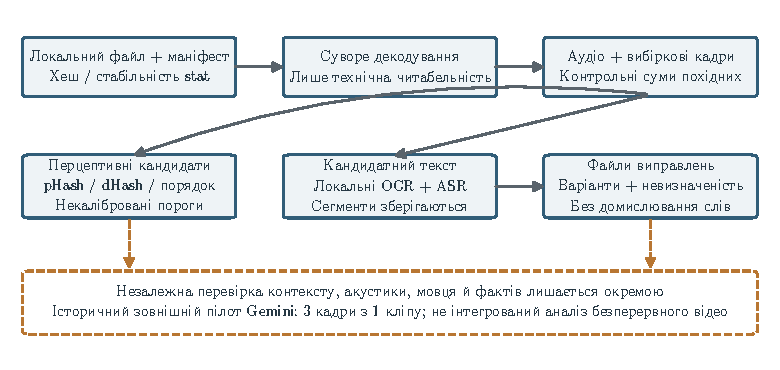
\includegraphics[width=\linewidth]{multimodal_pipeline.pdf}
\caption{Реалізований локальний мультимодальний конвеєр. Технічна обробка створює придатні для перегляду кандидатні спостереження. Незалежна акустична, контекстуальна, особова перевірка й перевірка подій є окремими завданнями; історичний зовнішній пілот Gemini на трьох ключових кадрах не входить до цього автоматизованого запускача.}
\label{fig:media}
\end{figure}

Порівняння вибіркових кадрів поєднує 63-бітний низькочастотний перцептивний хеш DCT і 64-бітний горизонтальний різницевий хеш. Воно оцінює повні кадри, кадри з обрізаною рамкою та центральні кадри, зокрема горизонтальні дзеркальні варіанти, і виключає малоінформативні кадри. Правило кандидатів за замовчуванням використовує межі Геммінга 10 і 12, щонайменше 0,6 часово узгодженого покриття коротшого проаналізованого вікна, три різні збіжні кадри й хеші та двосекундний проміжок. Зміщення найближчих кадрів і їхнє медіанне відхилення описують відносне вирівнювання послідовності. Ці розвідувальні пороги не є каліброваними ймовірностями збігу. Подібні накладення, статичні сцени та ефекти добору можуть давати хибнопозитивні результати; рідкісна вибірка, монтаж і кадрування --- хибнонегативні. Ані збіг, ані його відсутність не встановлюють місце запису, тотожність події, напрям копіювання чи автентичність.

\subsection{Кандидатне мовлення й текст}
Необов'язковий текстовий шлях використовує Tesseract OCR і faster-whisper ASR. OCR видає рамки слів і часові позначки, пов'язані з кадрами; ASR --- сегменти тексту з часом. Усталена архітектура OCR Tesseract і багатомовне навчання Whisper дають корисну основу для виділення тексту \citep{smith2007tesseract,radford2023whisper}. Їхні опубліковані результати не кількісно визначають роботу конкретних конвертованих моделей на українських, російських, змішаних за мовою чи зашумлених записах Social. Налаштування виконання й декодування faster-whisper також потребують явного версіонування \citep{systran2026faster}.

Історичні масові квитанції вказують CPU/int8 \code{Systran/faster-whisper-small}, ревізію \code{536b0662742c02347bc0e980a01041f333bce120} і faster-whisper 1.1.0. Обраний другий прохід по семи активах використовував \code{mobiuslabsgmbh/faster-whisper-large-v3-turbo}, ревізію \code{0a363e9161cbc7ed1431c9597a8ceaf0c4f78fcf}. Цей добір не є контрольованим порівнянням моделей на всьому корпусі. Початковий та альтернативний тексти зберігаються як супровідні файли виправлень; десять лексичних кандидатів у цьому перегляді лишаються \code{quote_safe=false}. Правдоподібного контекстуального формулювання недостатньо, щоб мовчки заповнювати нерозбірливе мовлення.

Безпека цитування має кілька окремих вимог: текст має відповідати аудіо, ім'я мовця має бути обґрунтованим, цитата має зберігати контекст, а фактичні твердження всередині цитати потребують власної оцінки доказів. Бенчмарк із 18 кліпів зберігає десять позначок \code{quote_safe=true}, але ідентифікатор ШІ-виконавця поряд із полем «людське акустичне прослуховування» незалежно не доводить участі людини-слухача. Наведено арифметику помилок відносно наданого еталона й зафіксовані позначки, а не незалежно перевірену безпеку цитування. Неочікувано вища помилка в номінальній страті чистого мовлення не може встановити загальний ефект шуму: кліпи, термінологія й побудова еталонів різняться, а кліпів у страті лише кілька.

\subsection{Здійсненність зовнішньої моделі та інтеграція}
Історична квитанція описує пілот користувацького Agy Gemini 3.8 Flash на трьох нерухомих кадрах з одного кліпу тривалістю 15,278 секунди. Спробу обробки повного відео заблоковано, а запуск на ключових кадрах повернув кандидатні візуальні спостереження. Це свідчення здійсненності виклику зовнішнього інструмента без валідації безперервного відео, аудіо, геолокації, особи, істинності чи точності. Поточний запускач Python не містить автоматичного виклику Gemini/Agy. Наведені кількості токенів не є виміряною грошовою вартістю, а результати іншої моделі не є незалежним підтвердженням сцени.
